\documentclass{beamer}

\usepackage{txfonts}
\usepackage{hyperref}
\usepackage{fancybox}
\usepackage{xfrac}
\usepackage{cancel}

\newcommand{\heart}{\ensuremath\heartsuit}

\usepackage{mathtools,amssymb}
\newcommand{\myarrow}{\scalebox{2}[2]{$\mathclap{\curvearrowleft}\mkern2.2mu
                                                 \mathclap{\curvearrowright}$}}



\hypersetup{colorlinks=false,linkbordercolor=red,linkcolor=green,pdfborderstyle={/S/U/W 1}}

\addtobeamertemplate{navigation symbols}{}{ \hspace{1em}    \usebeamerfont{footline}%
    \insertframenumber / \inserttotalframenumber}

\geometry{papersize={15cm,15cm}}
\usepackage{lipsum}

\makeatletter
\newenvironment<>{contdproof}[1][\proofname]{%
    \par
    \def\insertproofname{#1\@addpunct{.}}%
    \usebeamertemplate{proof begin}#2}
  {\usebeamertemplate{proof end}}
\makeatother


\setbeamertemplate{theorems}[numbered]

\newtheorem*{nonumdefinition}{Definition}
\newtheorem*{nonumproblem}{Problem}
\newtheorem*{nonumtheorem}{Theorem}
\newtheorem*{nonumremark}{Remark}
\newtheorem*{nonumremarks}{Remarks}
\newtheorem*{nonumexamples}{Examples}
\newtheorem*{nonumsolution}{Solution}
\newtheorem*{nonumexample}{Example}
\newtheorem*{nonumproposition}{Proposition}
\newtheorem{proposition}[theorem]{Proposition}


\usepackage{tikz}
\newcommand*\mycirc[1]{%
  \tikz[baseline=(C.base)]\node[draw,circle,inner sep=.7pt](C) {#1};\:
}

\newcommand\myheading[1]{%
  \par\bigskip
  {\color{blue}{\large #1}}\par\smallskip}

%\usetheme{Warsaw}
%\usetheme{Berkeley} %sample 1
\usetheme{Berlin} % sample 2
%\usetheme{AnnArbor} % sample 3

\let\otp\titlepage
\renewcommand{\titlepage}{\otp\addtocounter{framenumber}{-1}}

\title{Lecture 6 : Discrete Random Variables and Probability Distributions}
\author{}
\date{}

\begin{document}
\begin{frame}[plain]
\titlepage
\end{frame}

\begin{frame}
Go to ``BACKGROUND COURSE NOTES'' at the end of my web page and download the file {\it distributions}.

Today we say goodbye to the elementary theory of probability and start {\it Chapter 3}. We will open the door to the application of algebra to probability theory by introduction the concept of ``random variable''.
\end{frame}

\begin{frame}
What you will need to get from it (at a minimum) is the ability to do the following {\it ``Good Citizen Problems}''.

I will give you a {\em probability mass function} $P(X)$. You will be asked to compute 
\begin{itemize}
\item[(i)] The {\it expected value} (or {\it mean}) $E(X)$.

\item[(ii)] The {\it variance} $V(X)$.

\item[(iii)] The {\it cumulative distribution function} $F(x)$.
\end{itemize}
You will learn what these words mean shortly.
\end{frame}

\begin{frame}
\myheading{Mathematical Definition}

Let $S$ be the sample space of some experiment (mathematically a set $S$ with a probability measure $P$). A random variable $X$ is a real-valued function on $S$.

\myheading{Intuitive Idea}

A random variable is a function, whose values have probabilities attached.

\begin{nonumremark}
To go from the mathematical definition to the ``intuitive idea'' is tricky and not really that important at this stage.
\end{nonumremark}
\end{frame}

\begin{frame}
\myheading{The Basic Example}

Flip a fair coin three times so 
$$
S=\{HHH, \ HHT, \ HTH, \ HTT, \ THH, \ THT, \ TTH, \ TTT\}
$$
Let $X$ be function on $X$ given by
$$
X=\text{~number of heads}
$$
so $X$ is the function given by
\begin{center}
\begin{tabular}{r@{}cccccccc@{}l}
$\{$ & $HHH$, & $HHT$, & $HTH$, & $HTT$, & $THH$, & $THT$, & $TTH$, & $TTT$ & $\}$\\
     & $\downarrow$ & $\downarrow$ & $\downarrow$ & $\downarrow$ & $\downarrow$ & $\downarrow$ & $\downarrow$ & $\downarrow$\\
     & 3 & 2 & 2 & 1 & 2 & 1 & 1 & 0
\end{tabular}
\end{center}
What is
$$
P(X=0), \ P(X=3), \ P(X=1), \ P(X=2)
$$
\end{frame}

\begin{frame}
\myheading{Answers} Note $\sharp (S)=8$
\begin{align*}
P(X=0) &= P(TTT)=\dfrac{1}{8}\\
P(X=1) &= P(HTT)+P(THT)+P(TTH)=\dfrac{3}{8}\\
P(X=2) &= P(HHT)+P(HTH)+P(THH)=\sfrac{3}{8}\\
P(X=3) &= P(HHH)=\sfrac{3}{8}
\end{align*}
We will tabulate this
\begin{center}
\begin{tabular}{rc|c|c|c|c|}
Value & $X$ & $0$ & $1$ & $2$ & $3$\\
\cline{2-6}
Probability of the value & $P(X=x)$ & $\dfrac{1}{8}$ & $\dfrac{3}{8}$ & $\dfrac{3}{8}$ & $\dfrac{1}{8}$\\
\cline{2-6}
\end{tabular}
\end{center}
Get used to such tabular presentations.
\end{frame}

\begin{frame}
\myheading{Rolling a Die}

Roll a fair die, let
$$
X = \text{~the number that comes up}
$$
So $X$ takes values $1,2,3,4,5,6$ each with probability $\dfrac{1}{6}$.
\begin{center}
\begin{tabular}{c|c|c|c|c|c|c|}
$X$ & 1 & 2 & 3 & 4 & 5 & 6\\
\hline
$P(X=x)$ & $\dfrac{1}{6}$ & $\dfrac{1}{6}$ & $\dfrac{1}{6}$ & $\dfrac{1}{6}$ & $\dfrac{1}{6}$ & $\dfrac{1}{6}$\\
\hline
\end{tabular}
\end{center}
This is a special case of the {\it discrete uniform distribution} where $X$ takes values $1,2,3,\ldots,n$ each with probability $\dfrac{1}{n}$ (so roll a fair die with $n$ faces'').
\end{frame}

\begin{frame}
\myheading{Bernoulli Random Variable}

Usually random variables are introduced to make things numerical. We illustrate this by an important example - page 8. First meet some random variables.

\begin{nonumdefinition}[The simplest random variable(s)]
The actual simplest random variable is a random variable in the technical sense but isn't really random. It takes one value (let's suppose it is $0$) with probability one
\begin{center}
\begin{tabular}{c|c|}
$X$ & $0$\\
\hline
$P(X=0)$ & $1$\\
\hline
\end{tabular}
\end{center}
\end{nonumdefinition}
Nobody ever mentions this because it is too simple - it is deterministic.
\end{frame}

\begin{frame}
The simplest random variable that actually is random takes {\it TWO} values, let's suppose they are $1$ and $0$ with probabilities $p$ and $q$. Since $X$ has to be either $1$ on $0$ we must have
$$
p+q=1.
$$
So we get
\begin{center}
\begin{tabular}{c|c|c|}
$X$ & $1$ & $0$\\
\hline
$P(X=x)$ & $p$ & $q$\\
\hline
\end{tabular}
\end{center}
This called the {\it Bernoulli random variable with parameter $p$}. So a Bernoulli random  variable is a random variable that takes only {\it two} values $0$ and $1$.
\end{frame}

\begin{frame}
\myheading{Where do Bernoulli random variables come from?}

We go back to elementary probability.

\begin{nonumdefinition}
A {\it Bernoulli experiment} is an experiment which has two outcomes which we call (by convention) ``success'' $S$ and failure $F$.
\end{nonumdefinition}

\begin{nonumexample}
Flipping a coin. We will call a head a success and a toil a failure.

\smallskip

\dbend Often we call a ``success'' something that is in fact for from an actual success- e.g., a machine breaking down.
\end{nonumexample}
\end{frame}

\begin{frame}
By convention we let
$$
P(S)=p\quad\text{and}\quad P(F)=q
$$
so again $p+q=1$.

Thus the sample space $s$ of a Bernoulli experiment is given by
$$
s=\{S,F\}.
$$
To join up pages 7 and 9.

We define a random variable $X$ on $s$ by $X(S)=1$ and $X(F)=0$ so $P(X=1)=P(S)=p$ and $P(X=0)=P(F)=q$.
\end{frame}

\begin{frame}
\myheading{Discrete Random Variables}

\begin{nonumdefinition}
A subset $s$ of the red line $\mathbb{R}$ is said to be discrete if for every whole number $n$ there are only finitely many elements of $s$ in the interval $[-n,n]$.

\smallskip
\centerline{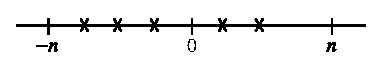
\includegraphics{figure/fig1.eps}}
\smallskip

So a {\it finite} subset of $\mathbb{R}$ is {\it discrete} but so is the set f integers $\mathbb{Z}$.
\end{nonumdefinition}
\end{frame}

\begin{frame}
\begin{nonumremark}
The definition in the text is wrong. The set of rational numbers $\mathbb{Q}$ is countably infinite but is not discrete. This is not important for this course.
\end{nonumremark}

\begin{nonumdefinition}
A random variable is said to be discrete if its set of possible values is a discrete set.
\end{nonumdefinition}

A possible value means a value $x_{0}$ so that $P(X=x_{0})\neq 0$.
\end{frame}

\begin{frame}
\begin{nonumdefinition}
The probability mass function (abbreviated proof) of a discrete random variable $X$ is the function $P_{X}$ defined by
$$
P_{X}(x)=P(X=x)
$$
We will often write $P(x)$ instead of $P_{X}(x)$.

Note
\begin{itemize}
\item[(i)] $P(x)\geq 0$

\item[(ii)] $\sum\limits_{\substack{\text{all possible}\\ X}} P(x)=1$

\item[(iii)] $P(x)=0$ for all $X$ outside a countable set.
\end{itemize}
\end{nonumdefinition}
\end{frame}

\begin{frame}
\myheading{Graphical Representations of Proof's}

There are two kinds of graphical representations of proof's, the ``line graph'' and the ``probability histogram''. We will illustrate them with the Bernoulli distribution with parameter $P$.
\begin{center}
\begin{tabular}{c|c|c|c}
$X$ & $1$ & $0$ &\\
\cline{1-3}
$P(X=x)$ & $P$ & $Q$ &\qquad table\\
\cline{1-3}
\end{tabular}
\end{center}
\centerline{~~~~~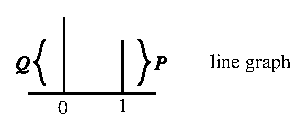
\includegraphics{figure/fig2.eps}}
\smallskip

\centerline{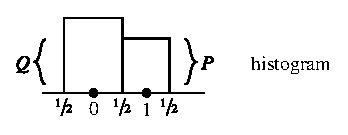
\includegraphics{figure/fig3.eps}}
\end{frame}

\begin{frame}
We also illustrate these for the basic example (pg. 5).
\begin{center}
\begin{tabular}{c|c|c|c|c|c}
$X$ & $0$ & $1$ & $2$ & $3$ &\\
\cline{1-5}
$P(X=x)$ & $\frac{1}{8}$ & $\frac{3}{8}$ & $\frac{3}{8}$ & $\frac{1}{8}$ & \qquad table\\
\cline{1-5}
\end{tabular}
\end{center}

\centerline{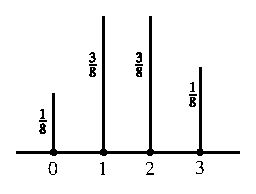
\includegraphics{figure/fig4.eps}}
\medskip

\centerline{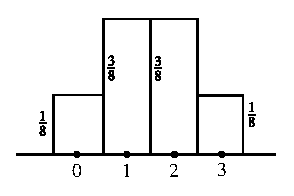
\includegraphics{figure/fig5.eps}}
\end{frame}

\begin{frame}
\myheading{The Cumulative Distribution Function}

The cumulative distribution function $F_{X}$ (abbreviated cdf) of a discrete random variable $X$ is defined by
$$
F_{X}(x)=P(X\leq x)
$$
We will often write $F(x)$ instead of $F_{X}(x)$.

\myheading{Bank account analogy}

Suppose you deposit 1000 at the beginning of every month.

\medskip

\centerline{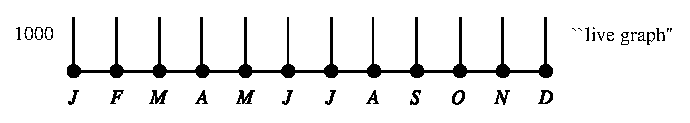
\includegraphics{figure/fig6.eps}}
\end{frame}

\begin{frame}
The ``line graph'' of you deposits is on the previous page. We will use $t$ (time as our variable). Let

$F(t)$ = the amount you have accumulated at time $t$.

What does the graph of $F$ look like?

\medskip

\centerline{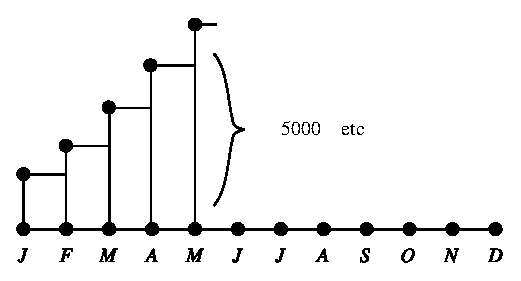
\includegraphics{figure/fig7.eps}}
\end{frame}

\begin{frame}
It is critical to observe that whereas the deposit function on page 15 is zero for all real numbers except 12 the cumulation function is never zero between 1 and $\infty$. You would be very upset if you walked into the bank on July $5^{\text{th}}$ and they told you your balance was zero - you never took any money out. Once your balance was nonzero it was never zero thereafter.
\end{frame}

\begin{frame}
\myheading{Back to Probability}

The cumulative distribution $F(x)$ is ``the total probability you have accumulated when you get to $x$''. Once it is nonzero it is never zero again ($P(x)\geq 0$ means ``you never take any probability out'').

To write out $F(x)$ in formulas you will need several (many) formulas. There should never be EQUALITIES in you formulas only INEQUALITIES.
\end{frame}

\begin{frame}
\myheading{The cdf for the Basic Example}

We have

\medskip
\centerline{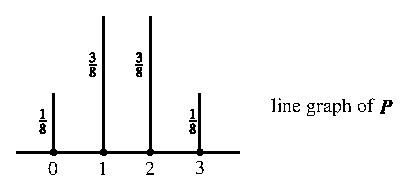
\includegraphics{figure/fig8.eps}}
\smallskip

So we start accumulation probability at $X=0$

\myheading{Ordinary Graph of $F$}

\smallskip
\centerline{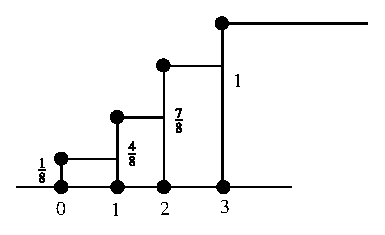
\includegraphics{figure/fig9.eps}}

\myheading{Formulas for $F$}
$$
\left\{
\begin{array}{cl}
0 & X\leq 0\\
\frac{1}{8} & 0\leq X<1\\[3pt]
\frac{4}{8} & 1\leq X<2\\[3pt]
\frac{7}{8} & 1\leq X<3\\[3pt]
1           & 3\leq X
\end{array} 
\right\} \quad \longleftarrow \text{ be careful}
$$
\end{frame}

\begin{frame}
You can see you here to be careful about the inequalities on the right-hand side.

\myheading{Expected Value}

\begin{nonumdefinition}
Let $X$ be a discrete random variable with set of possible values $D$ and pmf $P(x)$. The expected value or mean value of $X$ denote $E(X)$ or $\mu$ (Greek letter mu) is defined by 
$$
E (X)=\sum\limits_{x\in D}\times P(X=x)=\sum\limits_{x\in D}\times P(x)
$$
\end{nonumdefinition}
\end{frame}

\begin{frame}
\begin{nonumremark}
$E(X)$ is the whole point for monetary games of chance e.g., lotteries, blackjack, slot machines.

If $X$ = your payoff, the operators of these games make sure $E(X)<0$. Thorp's card-counting strategy in blackjack changed $E(X)<0$ (because tics went to the dealer) to $E(X)>0$ to the dismay of the casinos. See ``How to Beat the Dealer'' by Edward Thorp (a math professor of UCIrvine).
\end{nonumremark}
\end{frame}

\begin{frame}
\begin{nonumexamples}
The expicted value of the Bernoulli distribution.
\begin{align*}
E(X) &= \sum\limits_{x}\times P(X=x)=(0)(q)+(1)(P)\\
     &= P
\end{align*}
The expected value for the basic example (so the expected number of needs)
\begin{align*}
E(X) &= (0)\left(\dfrac{1}{8}\right)+(1)\left(\dfrac{3}{8}\right)+(2)\left(\dfrac{3}{8}\right)+(3)\left(\dfrac{1}{8}\right)\\[3pt]
     &= \dfrac{3}{2}
\end{align*}
\dbend The expected value is NOT the most probable value.
\end{nonumexamples}
\end{frame}

\begin{frame}
\begin{nonumexamples}[Cont.]
For the basic example the possible values of $X$ where $0$, $1$, $2$, $3$ so $\sfrac{3}{2}$ was not even a possible value
$$
P\left(X=\sfrac{3}{2}\right)=0
$$
The most probable values were $1$ and $2$ (tied) each with probability $\sfrac{3}{8}$.
\end{nonumexamples}

\myheading{Rolling of Die}
\begin{align*}
E(X) &= (1)\left(\dfrac{1}{6}\right)+(2)\left(\dfrac{1}{6}\right)+(3)\left(\dfrac{1}{6}\right)\\[3pt]
     &\quad +(4)\left(\dfrac{1}{6}\right)+(5)\left(\dfrac{1}{6}\right)+(6)\left(\dfrac{1}{6}\right)\\[3pt]
     &= \frac{1}{6}[1+2+3+4+5+6]=\frac{1}{\cancel{6}}\dfrac{\cancel{(7)(6)}}{2}\\[3pt]
     &= \sfrac{7}{3}.
\end{align*}
\end{frame}

\begin{frame}
\myheading{Variance}

The expected value does not tell you everything you went to know about a random variable (how could it, it is just one number). Suppose you and a friend play the following game of change. Flip a coin. If a head comes up you get \S1. If a toil comes up you pay your friend \S1. So if $X$ = your payoff.
\begin{gather*}
X(11)=+1, \ X(T)=-1\\[3pt]
E(X)=(+1)\left(\dfrac{1}{2}\right)+(-1)\left(\dfrac{1}{2}\right)=0
\end{gather*}
so this is a fair game.
\end{frame}

\begin{frame}
Now suppose you play the game changing \S1 to  \S1000. It is still a fair game
\begin{align*}
E(X) &= (1000)\left(\dfrac{1}{2}\right)+(-1000)\left(\dfrac{1}{2}\right)\\[3pt]
     &= 0
\end{align*}
but I personally would be very reluctant to play this game.

The notion of variance is designed to capture the difference between the two games.
\end{frame}

\begin{frame}
\begin{nonumdefinition}
Let $X$ be a discrete random variable with set of possible values $D$ and expected value $\mu$. Then the variance of $X$, denoted $V(X)$ or $\sigma^{2}$ (sigma squared) is defined by
\begin{align*}
V(X) &= \sum\limits_{x\in D}(x-\mu)^{2} P(X=x)\\[3pt]
     &= \sum\limits_{x\in D}(x-\mu)^{2}P(x)\tag{*}
\end{align*}
The standard deviation $\sigma$ of $X$ is defined to be the {\it square-root} of the variance
$$
\sigma = \sqrt{V(X)}=\sqrt{\sigma^{2}}
$$
\end{nonumdefinition}
\end{frame}

\begin{frame}
\begin{nonumdefinition}[Cont.]
Check that for the two games above (with your friend) 

$\sigma=1$ for the \S1 game

$\sigma=1000$ for the \S1000 game.
\end{nonumdefinition}

\myheading{The Shortcut Formula for $V(X)$}

The number of arithmetic operations (subtractions) necessary to compute $\sigma^{2}$ can be {\it greatly} reduced by using.

\begin{nonumproposition}
\begin{itemize}
\item[(i)] $V(X)=E(X^{2})-E(X)^{2}$

or

\item[(ii)] $V(X)=\sum\limits_{x\in D}X^{2}P(X)-\mu^{2}$
\end{itemize}
\end{nonumproposition}
\end{frame}

\begin{frame}
\begin{nonumproposition}[Cont.]
In the formula (*) you need $\sharp(D)$ subtractions (for each $x\in D$ you here to subtract $\mu$ then square ...). For the shortcut formula you need only one. {\it Always use} the shortcut formula.
\end{nonumproposition}

\begin{nonumremark}
Logically, version (i) of the shortcut formula is not correct because we haven't yet defined the random variable $X^{2}$.

We will do this soon - ``change of random variable''.
\end{nonumremark}
\end{frame}

\begin{frame}
\begin{nonumexample}[The fair die]
$X$ = outcome of rolling a die.

We have seen (pg. 24)
\begin{align*}
E(X) &= \mu=\dfrac{7}{2}\\[3pt]
E(X^{2}) &= (1)^{2}\left(\dfrac{1}{6}\right)+(2)^{2}\left(\dfrac{1}{6}\right)+(3)^{2}\left(\dfrac{1}{6}\right)\\[3pt]
        &\quad +(4)^{2}\left(\dfrac{1}{6}\right)+(5)^{2}\left(\dfrac{1}{6}\right)+(6)^{2}\left(\dfrac{1}{6}\right)\\[3pt]
        &=\frac{1}{6}\left[1^{2}+2^{2}+3^{2}+4^{2}+5^{2}+6^{2}\right]\\[3pt]
        &=\frac{1}{6}[91] \longleftarrow \text{later}
\end{align*}
So
$$
E(X^{2})=\dfrac{91}{6}
$$
Here

\medskip
\centerline{\includegraphics{figure/fig10.eps}}
\end{nonumexample}
\end{frame}

\begin{frame}
\begin{nonumremarks}
\begin{itemize}
\item[(1)] How did I know
$$
1^{2}+2^{2}+3^{2}+4^{2}+5^{2}+6^{2}=91
$$
This because
$$
\sum\limits^{n}_{k=1}k^{2}=\dfrac{n(n+1)(2x+1)}{6}
$$
Now plug in $n=6$.

\item[(2)] In the formula for $E(X^{2})$ {\it don't square} the probabilities

\medskip
\centerline{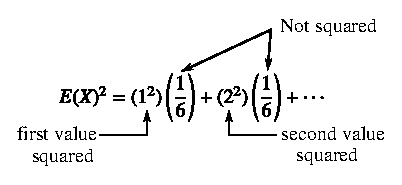
\includegraphics{figure/fig11.eps}}
\end{itemize}
\end{nonumremarks}
\end{frame}

\end{document}


